\documentclass{beamer}
\usetheme{Madrid}
\usepackage{amsmath}
\usepackage{xcolor}

\usepackage{graphicx}
\graphicspath{ {./images/} }

\title{Introduction to Deontological Ethics}
\author{Brendan Shea, PhD}
\date{Spring 2025}

\begin{document}

\begin{frame}
\titlepage
\end{frame}

\begin{frame}{Why Do Ethics Matter?}
\begin{itemize}
    \item Consider a doctor who could save five lives by harvesting organs from one healthy patient. Most would say this is wrong, but why exactly? Deontology offers an answer to such dilemmas.
    
    \item Our moral intuitions often align with rules rather than outcomes. When we say "the ends don't justify the means," we're thinking deontologically.
    
    \item Ethical frameworks shape everything from medical practices to artificial intelligence development, making their study crucial for modern challenges.
    
    \item Understanding deontology helps us evaluate whether actions are inherently right or wrong, regardless of their consequences.
\end{itemize}
\end{frame}

\begin{frame}{Deontology vs. Consequentialism}
\begin{itemize}
    \item \textbf{Deontology} (from Greek "deon" meaning duty): An ethical framework that judges the morality of actions based on their adherence to rules, duties, and obligations rather than their outcomes.
    
    \item \textbf{Consequentialism}: In contrast, judges actions solely by their consequences or outcomes, with the most famous version being utilitarianism's focus on maximum happiness for the maximum number.
    
    \item Deontologists believe certain actions are inherently wrong, even if they produce good consequences. Lying, for instance, violates human dignity and autonomy.
    
    \item The key difference lies in whether the ends can justify the means - deontology says no, consequentialism says yes.
\end{itemize}
\end{frame}

\begin{frame}{The Golden Rule}
\begin{itemize}
    \item \textbf{The Golden Rule}: "Do unto others as you would have them do unto you" appears across cultures and religions as a fundamental ethical principle.
    
    \item This rule aligns with deontological thinking by providing a universal standard for behavior that doesn't depend on calculating outcomes.
    
    \item The rule emphasizes moral reciprocity and helps us develop consistent ethical principles that could apply to everyone.
    
    \item It connects to Kant's \textbf{Categorical Imperative}: "Act only according to that maxim by which you can at the same time will that it should become a universal law."
\end{itemize}
\end{frame}

\begin{frame}{Historical Versions of the Golden Rule}
\begin{itemize}
   \item "What is hateful to you, do not do to your fellow: this is the whole Torah; the rest is the explanation; go and learn." 
   - Hillel the Elder, Babylonian Talmud, Shabbat 31a
   
   \item "Do not do to others what you would not want others to do to you."
   - Confucius, Analects 15:24
   
   \item "Treat your inferior as you would wish your superior to treat you."
   - Seneca, Letters to Lucilius, Letter 47
   
   \item "None of you truly believes until he wishes for his brother what he wishes for himself."
   - Prophet Muhammad, Hadith 13 of An-Nawawi
\end{itemize}
\end{frame}

\begin{frame}{Problems With the Golden Rule}
\begin{itemize}
    \item The Golden Rule assumes others have similar preferences and values to ourselves, which isn't always true. A masochist following this rule could justify causing pain to others.
    
    \item It can fail to account for power differentials and social positions. What I would want in my position might not apply to someone in very different circumstances.
    
    \item The rule doesn't help resolve conflicts between different people's desires or when multiple ethical principles clash.
    
    \item These limitations led to more sophisticated formulations like Kant's Categorical Imperative and modern human rights frameworks.
\end{itemize}
\end{frame}

\begin{frame}{Meet Immanuel Kant (1724-1804)}
\begin{itemize}
    \item Born in Königsberg, Prussia, Kant never traveled more than 40 miles from his hometown, yet his ideas revolutionized modern philosophy through rigorous intellectual exploration.
    
    \item Kant sought to ground morality in reason alone, arguing that ethical truths could be discovered through pure rational reflection, independent of religion or culture.
    
    \item His major ethical work, \textbf{Groundwork of the Metaphysics of Morals} (1785), attempts to identify and justify the supreme principle of morality.
    
    \item Despite his complex writing style, Kant believed moral truths should be accessible to all rational beings through careful reasoning.
\end{itemize}
\end{frame}

\begin{frame}{The Good Will}
\begin{itemize}
    \item \textbf{Good Will}: According to Kant, the only thing that is good without qualification - it remains good regardless of its consequences or the circumstances.
    
    \item Other seemingly good things (intelligence, courage, wealth) can become bad when paired with a bad will, but a good will remains intrinsically valuable even if it fails to achieve its aims.
    
    \item The good will is expressed through acting from duty (\textbf{aus Pflicht}) rather than merely in accordance with duty (\textbf{pflichtmäßig}). The motivation matters, not just the action.
    
    \item Example: A shopkeeper who gives correct change only to maintain reputation acts in accordance with duty, while one who does so because it's right acts from duty.
\end{itemize}
\end{frame}


\begin{frame}{What is a Categorical Imperative?}
\begin{itemize}
    \item \textbf{Hypothetical Imperatives} command conditionally: "If you want X, do Y." They depend on desires or goals and provide only conditional obligations.
    
    \item In contrast, the \textbf{Categorical Imperative} commands unconditionally: it tells us what we ought to do regardless of our desires or the consequences.
    
    \item Kant argues that moral commands must be categorical because morality's authority can't depend on contingent desires or outcomes - it must be necessary and universal.
    
    \item The Categorical Imperative has three main formulations, each highlighting different aspects of the same fundamental moral law.
\end{itemize}
\end{frame}

\begin{frame}{Kant on the Categorical Imperative}
\begin{itemize}
   \item "Act only according to that maxim by which you can at the same time will that it should become a universal law... Act as though the maxim of your action were by your will to become a universal law of nature."
   - Immanuel Kant, Groundwork of the Metaphysics of Morals (1785), 4:421
   
   \item "Act in such a way that you always treat humanity, whether in your own person or in the person of any other, never simply as a means, but always at the same time as an end."
   - Immanuel Kant, Groundwork of the Metaphysics of Morals (1785), 4:429
   
   \item "The moral law is holy (inviolable). Man is indeed unholy enough; but humanity in his person must be holy to him."
   - Immanuel Kant, Critique of Practical Reason (1788), 5:87
   
   \item "Two things fill the mind with ever new and increasing admiration and reverence... the starry heavens above me and the moral law within me."
   - Immanuel Kant, Critique of Practical Reason (1788), 5:161
\end{itemize}
\end{frame}

\begin{frame}{Universalizability Formula: Definition and Example}
\begin{itemize}
    \item First Formula: "Act only according to that maxim by which you can at the same time will that it should become a universal law." A \textbf{maxim} is your subjective principle of action.
    
    \item Example application: Consider lying to get out of a promise. Could you will that everyone act on the maxim "When convenient, break promises"? Such a world would make promising impossible.
    
    \item Some maxims fail because they create a \textbf{contradiction in conception} (like the promising example), while others create a \textbf{contradiction in will} (we couldn't rationally want them universalized).
    
    \item This formula helps identify moral laws by testing whether we could rationally will our maxims to become universal laws of nature.
\end{itemize}
\end{frame}

\begin{frame}{Graphic: Universalizability Formula}
% insert image

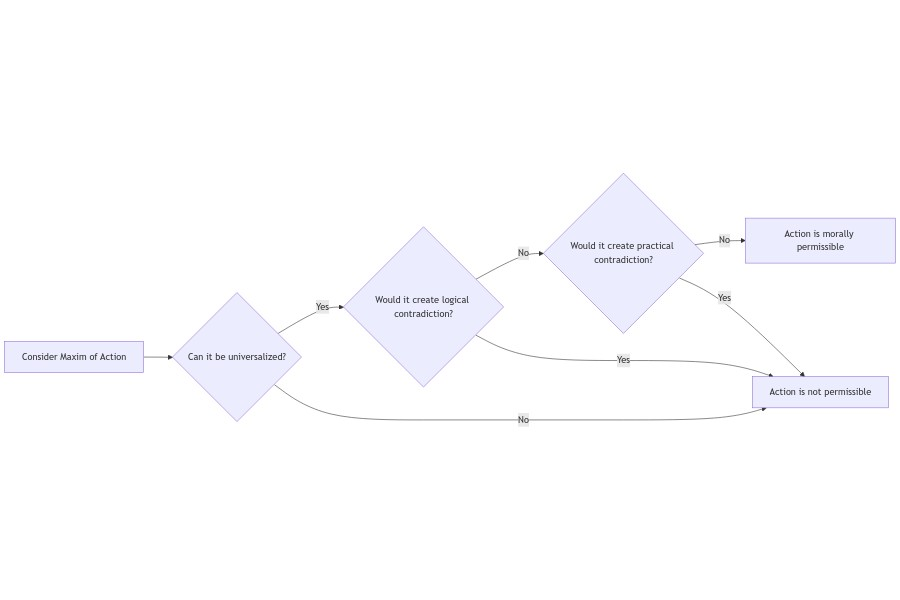
\includegraphics[scale=.35]{ci_universalize}

\end{frame}


\begin{frame}{Humanity Formula: Definition and Example}
\begin{itemize}
    \item Second Formula: "Act in such a way that you always treat humanity, whether in your own person or in the person of another, never simply as a means, but always at the same time as an end."
    
    \item \textbf{Treating as a Mere Means}: Using someone without their rational consent or in a way that ignores their capacity to set their own ends. Example: Making a false promise manipulates someone's rational agency.
    
    \item \textbf{Treating as an End}: Respecting others' capacity to set and pursue their own goals. This doesn't forbid all influence on others, but requires respecting their autonomy.
    
    \item Example application: Slavery is wrong because it treats humans as mere tools for others' purposes, denying their fundamental dignity as rational beings.
\end{itemize}
\end{frame}

\begin{frame}{Kingdom of Ends Formula: Definition and Example}
\begin{itemize}
    \item Third Formula: "Act according to the maxims of a universally legislating member of a merely possible kingdom of ends." A \textbf{Kingdom of Ends} is a systematic union of rational beings under common moral laws.
    
    \item This formula combines the universality of the first formula with the respect for persons of the second, imagining a moral community where everyone is both legislator and subject.
    
    \item Example application: When considering a maxim like "Exploit others' weaknesses for personal gain," ask whether this could be a law in an ideal moral community of rational beings.
    
    \item The Kingdom of Ends provides an ideal to strive for: a world where everyone's rational nature is respected and moral laws are universally recognized.
\end{itemize}
\end{frame}


\begin{frame}{Common Confusions About Kantian Ethics}
\begin{itemize}
    \item Confusion 1: "Kant prohibits all lying." Actually, Kant prohibits lying in the sense of making false promises or statements of fact, not all deception (like in games or fiction).
    
    \item Confusion 2: "Kantian ethics ignores consequences entirely." Rather, consequences matter but don't determine an action's moral worth; we must consider them when formulating maxims.
    
    \item Confusion 3: "The different formulas give different results." Kant insisted they were different expressions of the same fundamental law, though modern interpreters debate this.
    
    \item Confusion 4: "Kant's ethics are purely formal and empty." The formulas actually generate substantial moral constraints when properly applied to concrete maxims.
\end{itemize}
\end{frame}


\begin{frame}{Criticism: Is Universalization Too Abstract?}
\begin{itemize}
    \item The universalization test asks us to imagine our maxim becoming a universal law of nature - but how exactly do we describe these maxims? The level of description seems arbitrary.
    
    \item For example, consider lying to protect someone from harm. Is the maxim "Lie whenever convenient" or "Lie to protect innocent life" or "Lie to Nazi officers asking about hidden Jews"? Each leads to different results.
    
    \item Kant's theory seems to give different answers depending on how specifically or generally we describe the action. This makes the universalization test feel like a shell game where we can get whatever answer we want.
    
    \item Response: While this is a serious challenge, we might focus on the intention behind the action when formulating maxims. We should ask: "What principle am I really acting on here?"
\end{itemize}
\end{frame}

\begin{frame}{Criticism: Can We Really Separate Motives from Consequences?}
\begin{itemize}
    \item Kant insists that an action's moral worth comes purely from acting from duty, not from its consequences. But this seems to conflict with how we actually think about ethics.
    
    \item Consider a doctor who saves lives only from duty, feeling no compassion or care for patients, versus one who acts from both duty and compassion. Kant's view suggests the first doctor acts more morally.
    
    \item This separation of duty from natural feelings and good consequences seems psychologically unrealistic and potentially harmful - do we really want doctors, parents, or friends acting purely from duty?
    
    \item Response: Perhaps Kant's point is not that we should eliminate natural feelings, but that duty must be able to override them when they conflict with what's right. Compassion can complement duty.
\end{itemize}
\end{frame}

\begin{frame}{Rossian Pluralism: Overview}
\begin{itemize}
    \item \textbf{Moral Pluralism}: W.D. Ross argued that there isn't just one supreme moral principle (like Kant's Categorical Imperative), but several distinct, irreducible moral duties.
    
    \item These duties are \textbf{prima facie} (at first glance) rather than absolute - they can be outweighed by other duties in specific situations, but never simply disappear.
    
    \item Ross believes these duties are self-evident through moral reflection, like mathematical truths. We discover rather than construct them through careful consideration of our moral intuitions.
    
    \item This approach tries to capture the complexity of moral life while maintaining objective moral truth - different duties can pull us in different directions.
\end{itemize}
\end{frame}

\begin{frame}{Graphic: Rossian Pluralism}
    % insert image
    
    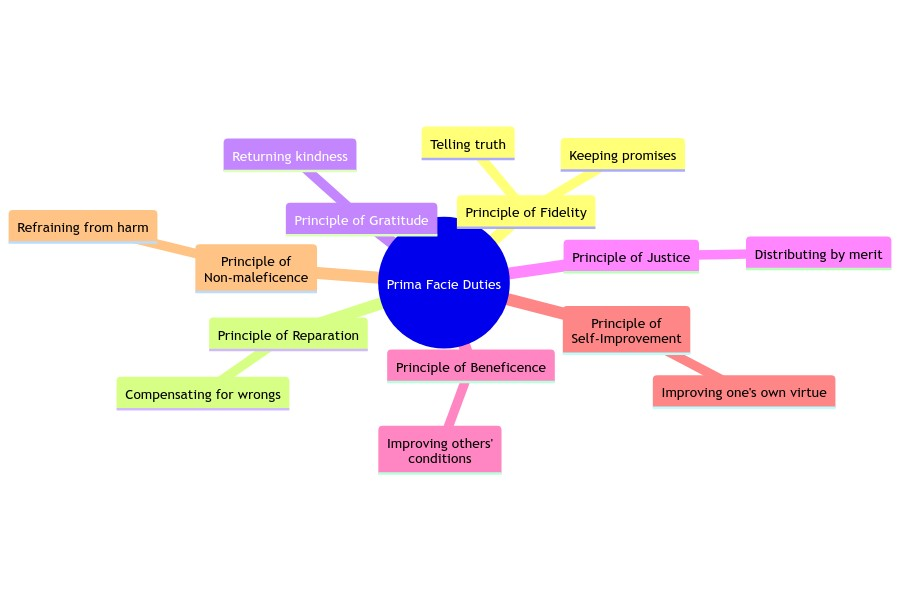
\includegraphics[scale=.35]{ross_pluralism.png}
    
    \end{frame}

\begin{frame}{Prima Facie Duties: Fidelity and Reparation}
\begin{itemize}
    \item \textbf{Duty of Fidelity}: We have a duty to keep promises and be truthful. This arises from explicit promises and implicit commitments we make through our words and actions.
    
    \item The strength of this duty varies with the solemnity and explicitness of the promise - a casual "see you later" carries less weight than a marriage vow.
    
    \item \textbf{Duty of Reparation}: We have a duty to make amends for harms or wrongs we've caused to others, whether intentional or unintentional.
    
    \item This duty includes both material compensation and moral repair (like apology and reconciliation), aiming to restore relationships and right past wrongs.
\end{itemize}
\end{frame}

\begin{frame}{Prima Facie Duties: Gratitude and Justice}
\begin{itemize}
    \item \textbf{Duty of Gratitude}: We have obligations to those who have helped or benefited us. This includes acknowledging help, showing appreciation, and returning favors when appropriate.
    
    \item The strength of this duty varies with the magnitude of the benefit and the sacrifice or effort involved in providing it.
    
    \item \textbf{Duty of Justice}: We have an obligation to distribute benefits and burdens fairly, ensure people get what they deserve, and prevent unearned advantages or disadvantages.
    
    \item Justice includes both retributive aspects (responding to wrongs) and distributive aspects (fair allocation of resources and opportunities).
\end{itemize}
\end{frame}

\begin{frame}{Prima Facie Duties: Beneficence and Self-Improvement}
\begin{itemize}
    \item \textbf{Duty of Beneficence}: We have a positive duty to help others and promote their wellbeing when we can do so without excessive cost to ourselves.
    
    \item This duty extends beyond just helping those who have helped us, but its strength varies with our relationship to others and our capacity to help.
    
    \item \textbf{Duty of Self-Improvement}: We have an obligation to develop our talents, knowledge, and moral character to become better people and more capable of fulfilling other duties.
    
    \item This includes both intellectual and moral development - we should strive to improve our understanding and our ability to recognize and respond to moral situations.
\end{itemize}
\end{frame}

\begin{frame}{Prima Facie Duties: Non-Maleficence and Special Relations}
\begin{itemize}
    \item \textbf{Duty of Non-Maleficence}: We have a duty not to harm others. Ross argues this is distinct from beneficence and often stronger - the duty not to harm typically outweighs the duty to help.
    
    \item This includes avoiding both direct harm and creating circumstances likely to lead to harm. Mental and emotional harms count alongside physical ones.
    
    \item \textbf{Duties from Special Relations}: We have special obligations to family, friends, colleagues, and others with whom we share particular relationships or roles.
    
    \item These relationship-based duties often take precedence over more general duties to humanity at large, though they don't completely override them.
\end{itemize}
\end{frame}

\begin{frame}{Example Application of Rossian Pluralism}
\begin{itemize}
    \item Consider: You promised to meet a friend for coffee, but on the way you witness a minor accident. Stopping to help means breaking your promise.
    
    \item Relevant duties: Fidelity (keeping the promise), Beneficence (helping accident victims), Non-maleficence (preventing potential harm from lack of assistance).
    
    \item The prima facie duty of beneficence here likely outweighs fidelity because the potential harm from not helping exceeds the harm of a broken promise.
    
    \item The broken promise doesn't disappear - you still owe your friend an explanation and perhaps reparation (like rescheduling), showing how multiple duties remain relevant.
\end{itemize}
\end{frame}

\begin{frame}{Common Confusions About Pluralism}
\begin{itemize}
    \item Confusion 1: "Prima facie duties are just rules of thumb." Actually, they are genuine moral obligations that retain their force even when outweighed - unlike mere rules of thumb.
    
    \item Confusion 2: "Ross's system lacks any way to rank or prioritize duties." While there's no absolute ranking, Ross provides guidelines based on the strength and specificity of obligations.
    
    \item Confusion 3: "Moral pluralism means moral relativism." Ross believes these duties are objective moral truths we discover through reflection, not subjective or cultural constructs.
    
    \item Confusion 4: "If duties conflict, one must be false." Rather, both duties remain valid even when one outweighs the other in a specific situation.
\end{itemize}
\end{frame}

\begin{frame}{Criticism: Does Pluralism Give Us Real Guidance?}
\begin{itemize}
    \item Unlike Kantian ethics or utilitarianism, Ross's theory provides no single principle or decision procedure for resolving conflicts between duties. We must rely on judgment and intuition.
    
    \item In complex situations where multiple duties conflict, the theory seems to just tell us to "think carefully and do what seems right" - but isn't this what we were doing anyway?
    
    \item This lack of systematic guidance can be especially problematic in novel situations or when reasonable people disagree about which duty should take precedence.
    
    \item Response: Perhaps this accurately reflects the real complexity of moral life. A theory that provides clear answers in all cases might be suspiciously oversimplified.
\end{itemize}
\end{frame}

\begin{frame}{Criticism: Are These Really All The Duties?}
\begin{itemize}
    \item Ross claims his list of duties is complete and self-evident, discovered through careful moral reflection. But why these particular duties and not others?
    
    \item Some argue for additional duties not on Ross's list, such as duties to the environment, to future generations, or to preserve cultural heritage. Ross's method gives no clear way to evaluate these claims.
    
    \item The duties seem to reflect the moral intuitions of an early 20th century British academic. Different cultures and times might "self-evidently" discover different fundamental duties.
    
    \item Response: The framework could potentially accommodate new duties while maintaining its core insight that morality involves multiple irreducible principles.
\end{itemize}
\end{frame}

\begin{frame}{Threshold Deontology: Overview}
\begin{itemize}
    \item \textbf{Threshold Deontology}: A hybrid theory that follows deontological rules up to a certain threshold of consequences, beyond which consequentialist considerations take over.
    
    \item Below the threshold, actions are governed by moral rules or constraints regardless of consequences - similar to traditional deontology.
    
    \item Above the threshold, when consequences become severe enough, the theory allows violation of these normally binding rules to prevent disaster.
    
    \item This approach tries to capture both our intuition that some actions are simply wrong and our feeling that rules might be broken to prevent catastrophes.
\end{itemize}
\end{frame}

\begin{frame}{Graphic: Threshold}
    % insert image
    
    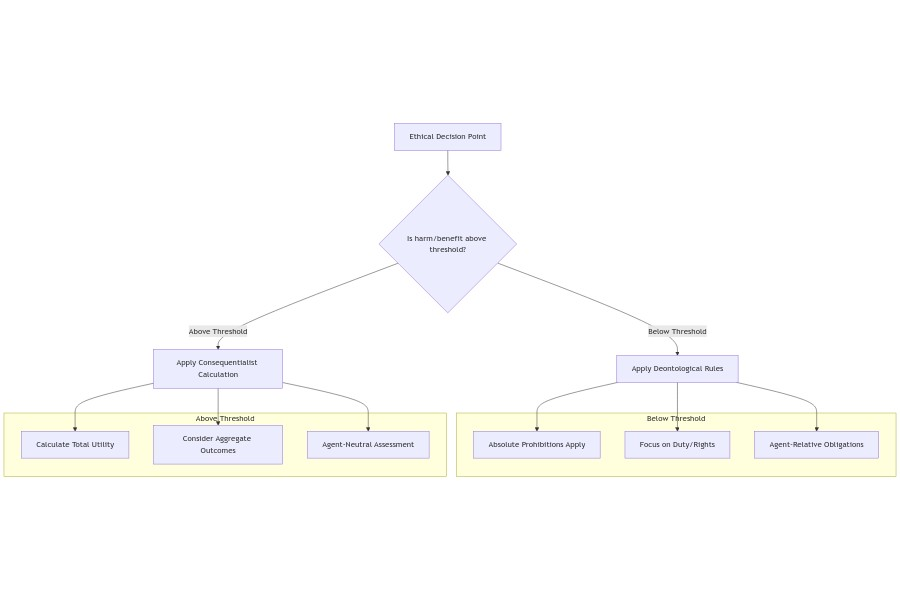
\includegraphics[scale=.35]{threshold.png}
    
    \end{frame}

\begin{frame}{Below the Threshold: Moral Side Constraints}
\begin{itemize}
    \item \textbf{Side Constraints}: Absolute prohibitions that limit what we can do in pursuit of good consequences, functioning as "moral boundaries" we normally cannot cross.
    
    \item Examples include prohibitions on murder, torture, and using people merely as means - actions that violate basic human dignity and rights.
    
    \item These constraints apply even when violating them would produce better consequences, reflecting the idea that some actions are inherently wrong.
    
    \item The constraints protect individual rights and dignity from being sacrificed for the greater good in ordinary circumstances.
\end{itemize}
\end{frame}

\begin{frame}{More Side Constraints}
\begin{itemize}
    \item \textbf{Constraint Against Coercion}: We may not force people to act against their will, even if coercion would lead to better outcomes for them or others.
    
    \item \textbf{Constraint Against Deception}: We may not deliberately deceive others or manipulate their understanding of reality, even for seemingly beneficial ends.
    
    \item \textbf{Constraint Against Promise-Breaking}: We must keep our commitments even when breaking them would produce better consequences, barring extreme circumstances.
    
    \item These constraints reflect basic respect for human autonomy and rationality, protecting people's ability to make their own choices.
\end{itemize}
\end{frame}

\begin{frame}{What is a Threshold?}
\begin{itemize}
    \item A threshold represents the point at which the negative consequences become so severe that they override normal deontological constraints. But how do we determine this point?
    
    \item \textbf{Quantitative Thresholds}: Some argue for specific numbers (e.g., violate a constraint to save 100 lives). However, this raises questions about why that particular number.
    
    \item \textbf{Qualitative Thresholds}: Others argue for qualitative differences (e.g., preventing civilization-ending catastrophes). This avoids arbitrary numbers but may be too vague.
    
    \item The threshold must be high enough to preserve the force of moral rules in ordinary cases, but not so high as to seem fanatical in the face of disaster.
\end{itemize}
\end{frame}

\begin{frame}{Beyond the Threshold}
\begin{itemize}
    \item Once we cross the threshold, consequentialist reasoning takes over - we should choose whatever action produces the best outcomes, even if it violates normal moral rules.
    
    \item However, the violation of moral rules still matters - it leaves what philosophers call \textbf{moral residue}, requiring regret, compensation, and reparation where possible.
    
    \item The shift to consequentialism doesn't mean "anything goes" - we should still choose the least morally problematic way to achieve the necessary outcomes.
    
    \item After the emergency passes, we return to respecting normal moral constraints. The threshold represents an exception, not a permanent abandonment of moral rules.
\end{itemize}
\end{frame}

\begin{frame}{Example Applications of Threshold Deontology}
\begin{itemize}
    \item The Ticking Bomb Scenario: Should we torture one terrorist to prevent a nuclear explosion? Threshold deontology suggests yes, while acknowledging the serious wrong of torture.
    
    \item Medical Triage in Disasters: When resources are extremely limited, we might abandon normal medical ethics of consent and fairness in favor of saving the most lives possible.
    
    \item Military Decisions: Targeting civilians is normally forbidden, but might be justified to prevent genocide or nuclear war. The threshold helps explain when such violations become permissible.
    
    \item Pandemic Response: Individual rights to movement and assembly might be overridden to prevent massive death tolls, though this requires a very high threshold.
\end{itemize}
\end{frame}

\begin{frame}{Common Confusions About Threshold Deontology}
\begin{itemize}
    \item Confusion 1: "It's just rule consequentialism in disguise." No - it genuinely treats moral rules as binding below the threshold, not just as rules of thumb for producing good consequences.
    
    \item Confusion 2: "Once we cross the threshold, anything is permitted." False - we still aim to minimize violations and choose the least problematic ways to achieve necessary outcomes.
    
    \item Confusion 3: "It's purely subjective when to cross the threshold." While there's room for disagreement, the theory provides frameworks for reasoning about thresholds based on severity and scope of consequences.
    
    \item Confusion 4: "It's inconsistent to switch between moral frameworks." The theory sees this as a feature, not a bug - it reflects our considered moral judgments about both rules and consequences.
\end{itemize}
\end{frame}

\begin{frame}{Criticism: The Arbitrariness Problem}
\begin{itemize}
    \item Unlike pure deontology or pure consequentialism, Threshold Deontology seems to give us two different moral frameworks with no principled reason for switching between them.
    
    \item If consequences matter enough to override moral rules in extreme cases, why don't they matter in ordinary cases? What justifies this sudden switch in moral reasoning?
    
    \item The choice of threshold seems arbitrary - whether quantitative (save 100 lives) or qualitative (prevent catastrophe). Why this threshold rather than a higher or lower one?
    
    \item Response: Perhaps the threshold reflects a real feature of moral life - just as water changes state at certain temperatures, moral reasoning might naturally shift at certain levels of severity.
\end{itemize}
\end{frame}

\begin{frame}{Criticism: The Incentive Problem}
\begin{itemize}
    \item If we publicly acknowledge that moral rules can be broken in extreme circumstances, this might create perverse incentives for bad actors to manufacture "emergencies."
    
    \item Consider terrorists who deliberately create situations that cross the threshold, knowing this will force us to negotiate or compromise our principles.
    
    \item Even well-intentioned people might be tempted to exaggerate the severity of situations to justify breaking moral rules they find inconvenient.
    
    \item Response: This is a serious practical concern, but keeping thresholds very high and emphasizing the continued wrongness of rule violations might help mitigate these risks.
\end{itemize}
\end{frame}

\begin{frame}{Review: Three Approaches to Deontology}
\begin{itemize}
    \item \textbf{Kantian Deontology}: Emphasizes absolute moral rules derived from reason alone, focused on respect for rational nature and universal laws. Struggles with apparent conflicts between duties.
    
    \item \textbf{Rossian Pluralism}: Recognizes multiple irreducible moral duties that can conflict. More flexible than Kant but provides less systematic guidance for resolving conflicts.
    
    \item \textbf{Threshold Deontology}: Attempts to combine deontological rules with consequentialist considerations in extreme cases. More practical but faces challenges about arbitrariness.
    
    \item Each approach captures important moral intuitions while facing distinct theoretical and practical challenges.
\end{itemize}
\end{frame}

\begin{frame}{Review: Key Insights and Challenges}
\begin{itemize}
    \item Key Insight 1: Some actions seem wrong regardless of consequences - deontology captures our intuition that the ends don't always justify the means.
    
    \item Key Insight 2: Moral life involves multiple types of obligations that can conflict - no single principle can capture all of morality.
    
    \item Key Challenge 1: How do we handle apparent conflicts between moral rules or duties? Different forms of deontology answer this differently.
    
    \item Key Challenge 2: How do we balance respect for moral rules with preventing catastrophic outcomes? This remains a central tension in deontological ethics.
\end{itemize}
\end{frame}

\begin{frame}{Discussion Question 1: The Trolley Problem Revisited}
\begin{itemize}
    \item Consider the classic trolley problem: A runaway trolley is headed toward five people. You can pull a lever to divert it to another track, where it will kill one person instead.
    
    \item How would each version of deontology approach this?
    \begin{itemize}
        \item Kantian: Does diverting violate the Humanity Formula? 
        \item Rossian: Which prima facie duties are relevant?
        \item Threshold: Is five lives enough to cross the threshold?
    \end{itemize}
        
    \item Does adding details change the analysis? What if the one person is a doctor who could save hundreds? What if the five people are terminally ill?
    
    \item This raises deeper questions about moral mathematics: Can we really weigh lives against each other? Does intention matter more than outcomes?
\end{itemize}
\end{frame}

\begin{frame}{Discussion Question 2: AI and Deontological Constraints}
\begin{itemize}
    \item Imagine programming an autonomous AI system. Should we give it strict deontological rules ("never lie") or allow for threshold-based flexibility in extreme cases?
    
    \item What are the risks of each approach? 
    \begin{itemize}
        \item Strict rules might lead to disaster in unexpected situations
        \item Flexible rules might be manipulated or misinterpreted
    \end{itemize}
        
    \item How would different deontological frameworks handle AI decision-making?
    \begin{itemize}
        \item Could an AI system truly understand and apply the Categorical Imperative?
        \item Could it weigh prima facie duties like a human?
    \end{itemize}
        
    \item This connects to broader questions about moral judgment: Can moral decision-making be reduced to rules and algorithms, or does it require human wisdom?
\end{itemize}
\end{frame}
\end{document}